\documentclass[../nirs.tex]{subfiles}

\begin{document}
\section{Описание выходной информации: сигналов, документов и видеокадров}
Выходной информацией в разрабатываемой системе является:

\begin{enumerate}

    \item График прохождения технических осмотров -- содержит календарный график
        прохождения технического осмотра каждой единицей техники (рисунок
        \ref{fig:design-calendar}).

        \begin{figure}[H]
        \centering
        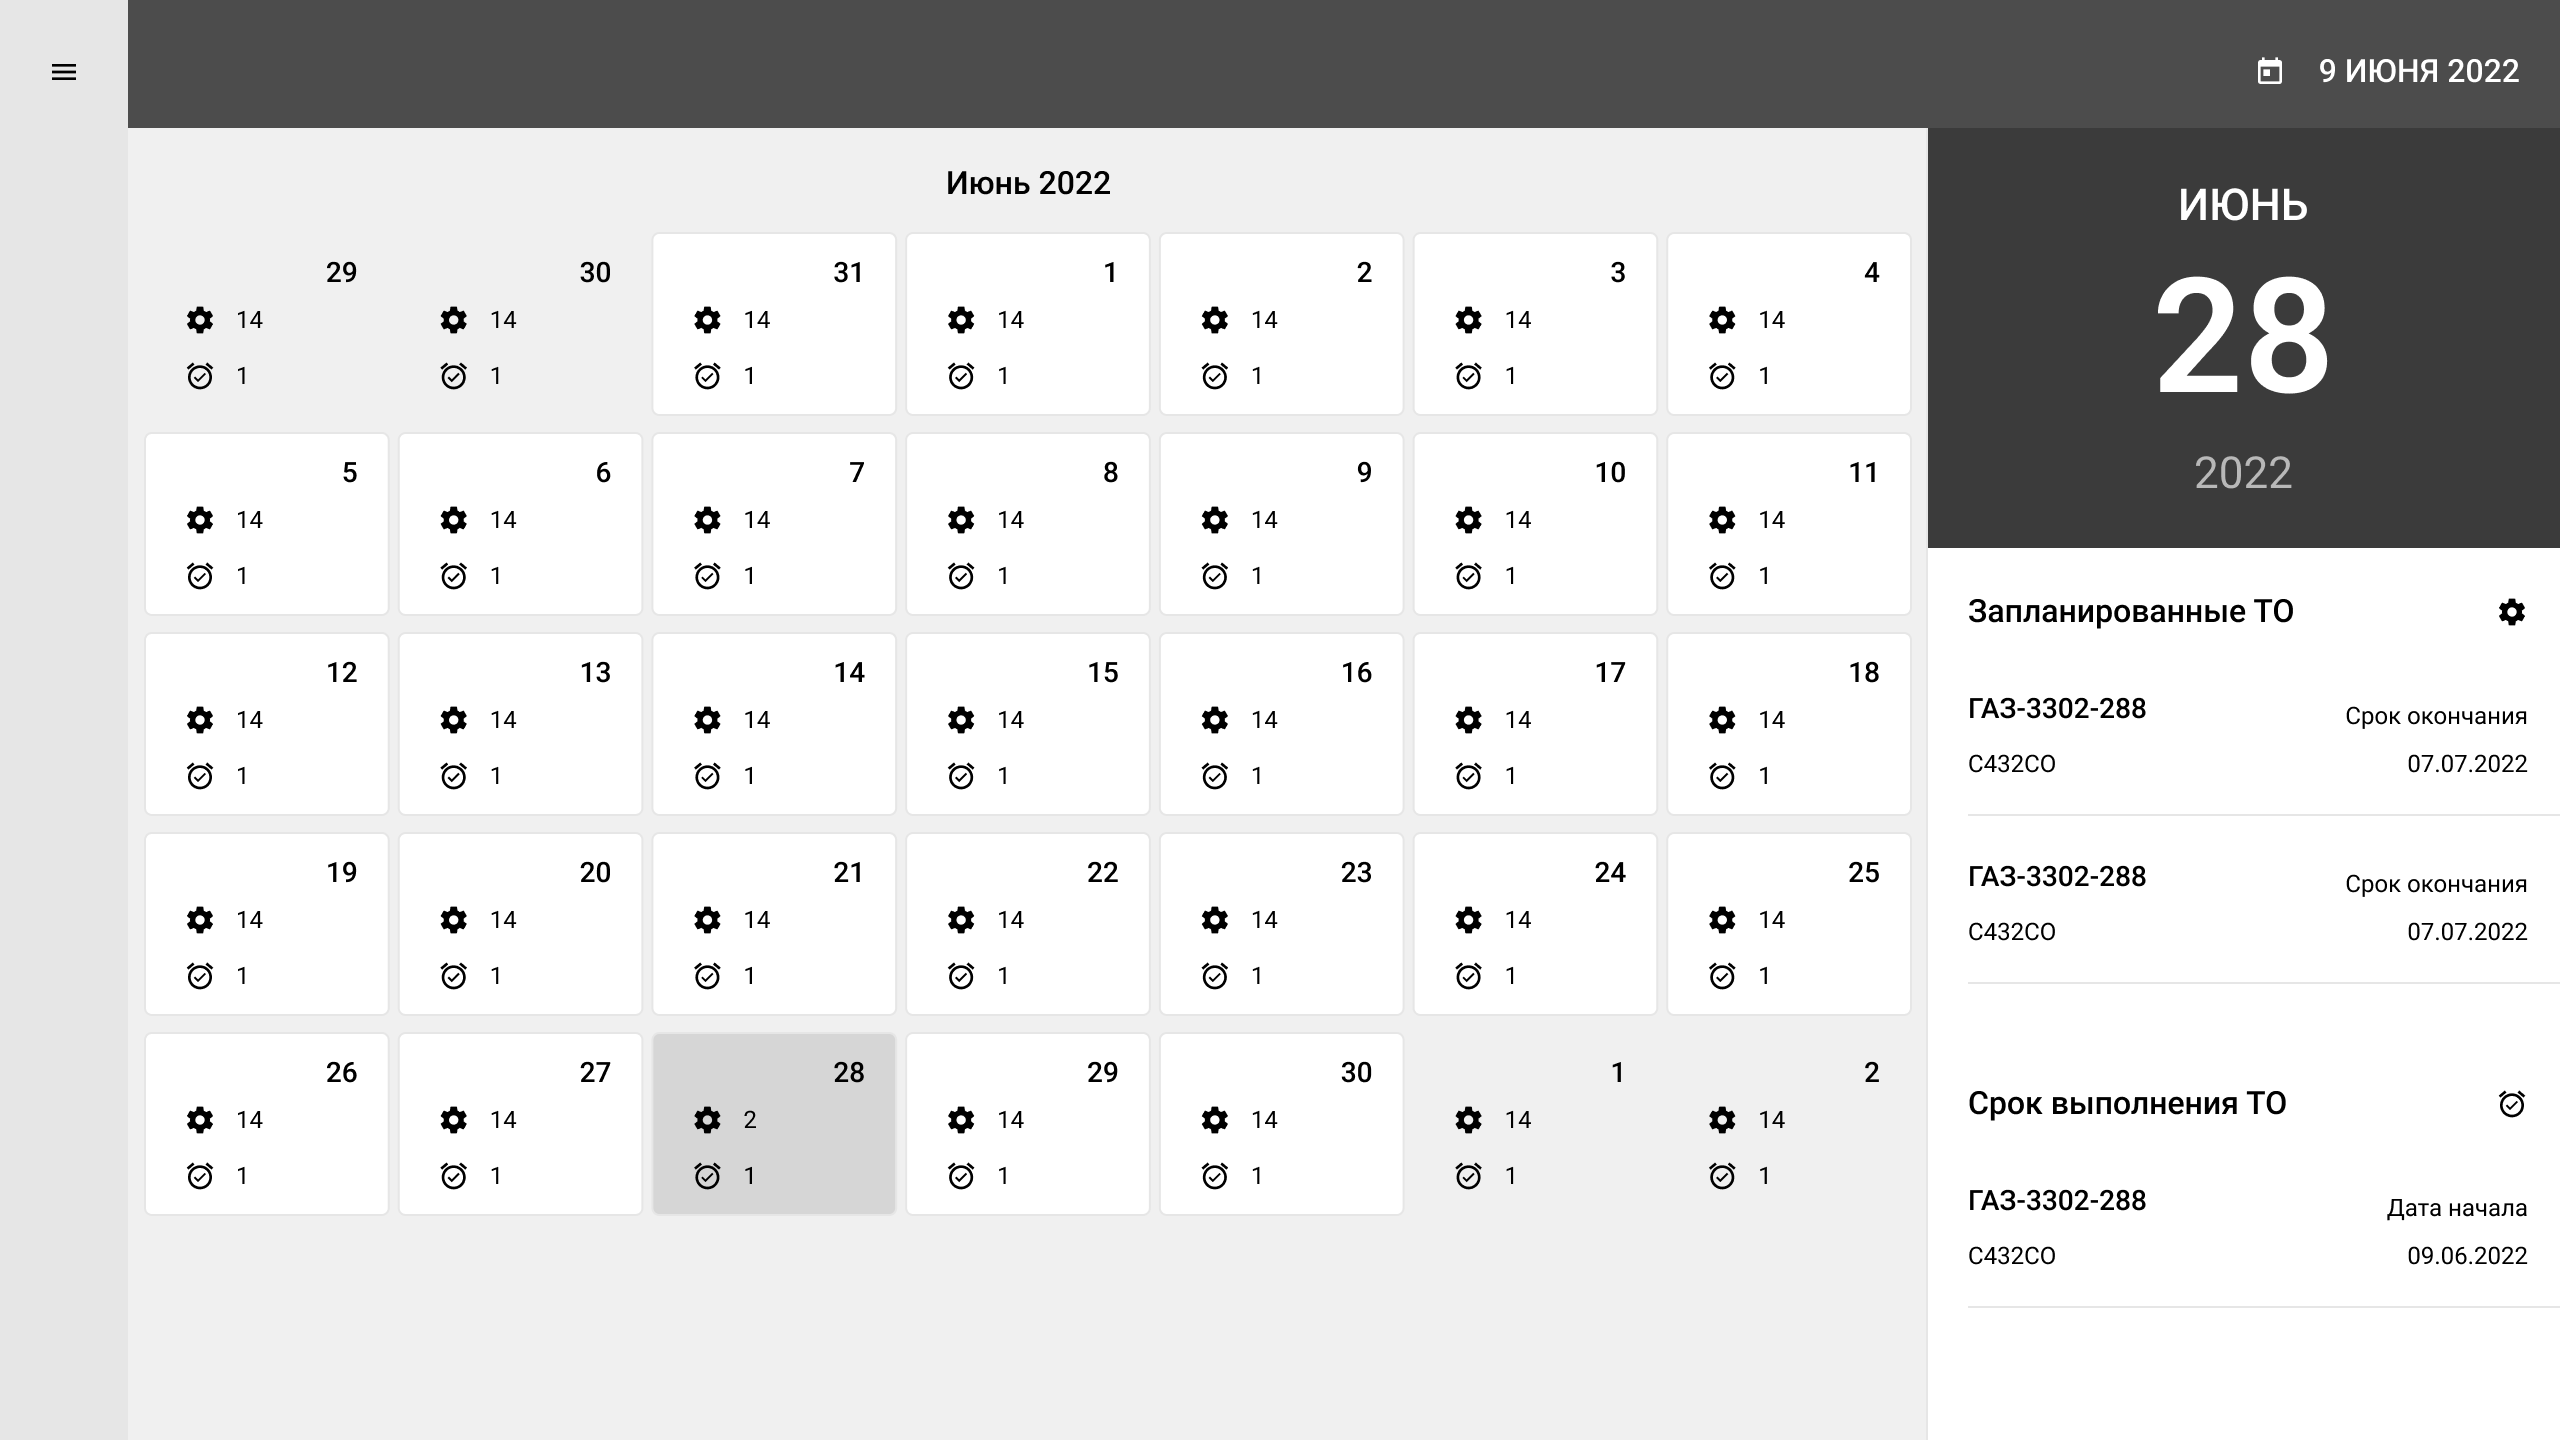
\includegraphics[keepaspectratio,width=\textwidth]{./images/calendar-planning.png}
        \caption{Макет экрана графика прохождения технических осмотров
        разрабатываемой системы}
        \label{fig:design-calendar}
        \end{figure}

	\item Отчеты по затратам -- содержат информацию о количестве расходов в
		рамках заданного пользователем временного промежутка (рисунок
        \ref{fig:design-report}).

        \begin{figure}[H]
        \centering
        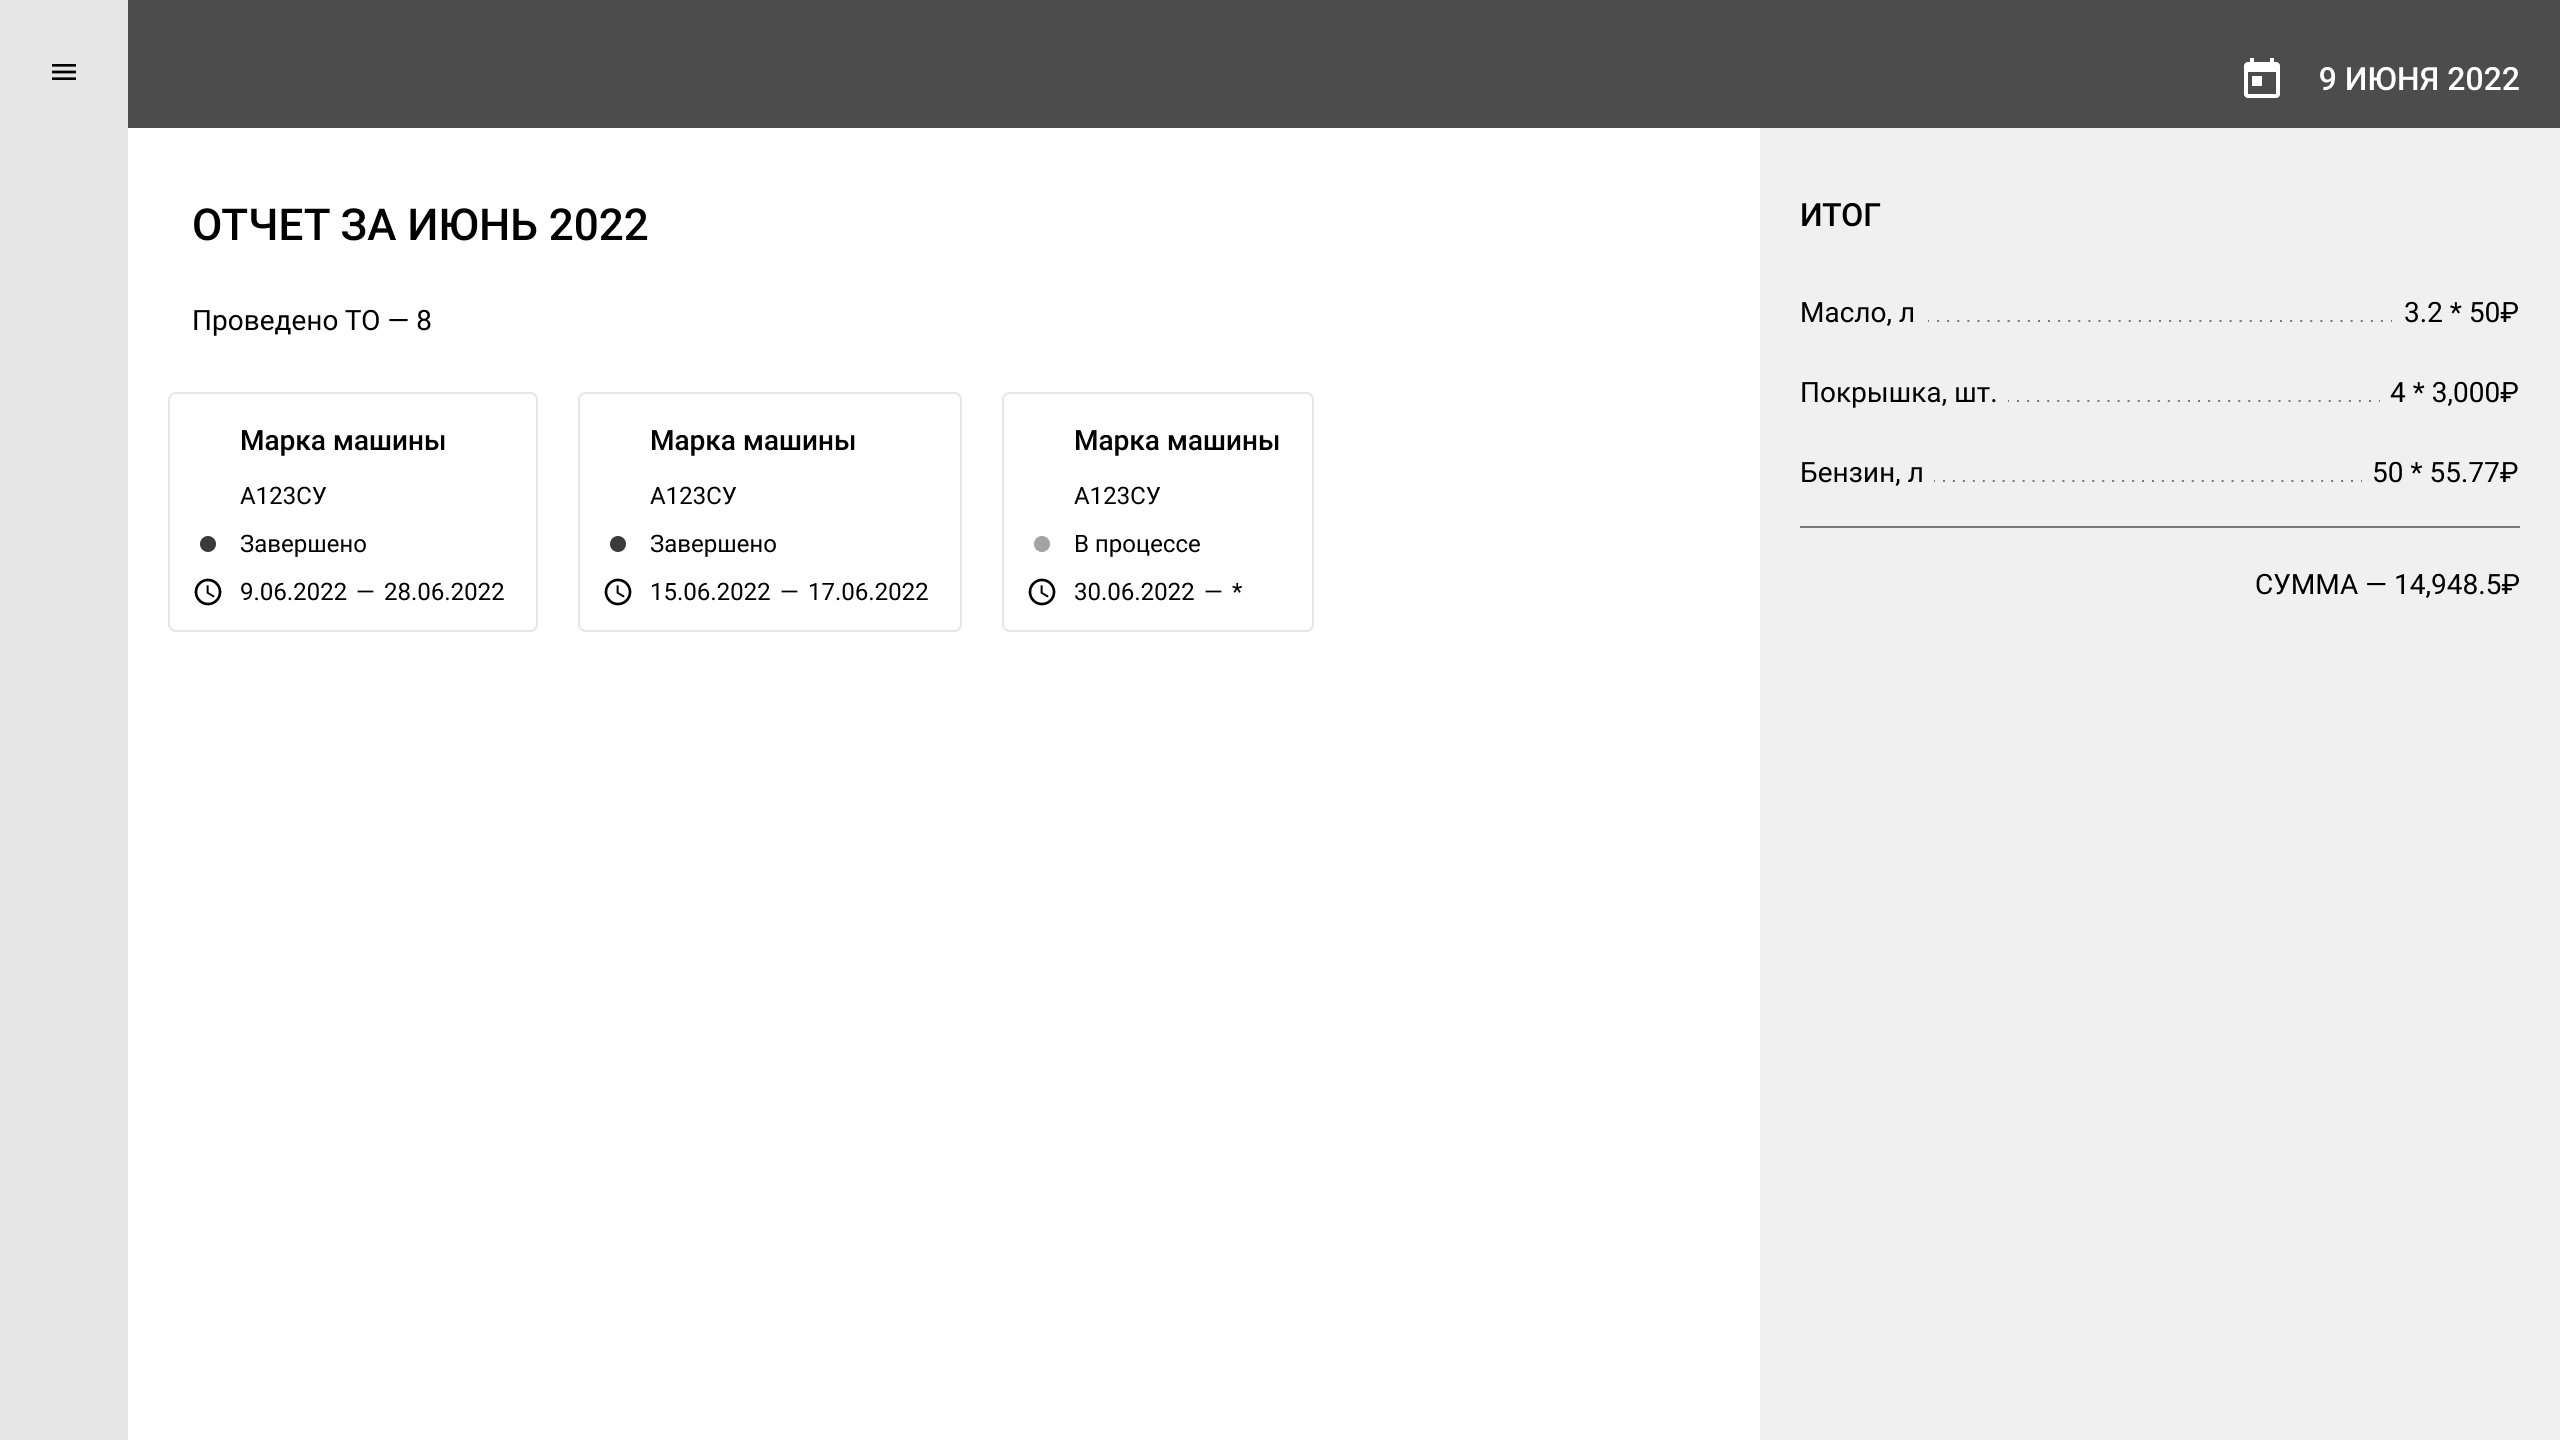
\includegraphics[keepaspectratio,width=\textwidth]{./images/expenses-report.png}
        \caption{Макет экрана отчета по затратам разрабатываемой системы}
        \label{fig:design-report}
        \end{figure}
\end{enumerate}
\end{document}
